\newpage
\section{Description of Models}
This section presents a description of a number of models, including the wheel unit, wheel unit subsystem and the central unit in both duplex and triplex configuration (See the Central unit section). In addition their respective reliability block diagrams and fault trees are presented.

The wheel unit consists of a number of subunits. It uses two fail-silent computer modules, two sensors, one actuator and four 
bus interfaces (hänvisning till bild). The failure rate and coverage for each of these subunits in are given in the table from the previous section. These values also differ depending on the architecture. Seen below is a figure of the wheel unit and its corresponding reliability block diagram.

\subsection{Wheel Unit Model}
\begin{figure}[H]
  \centering
  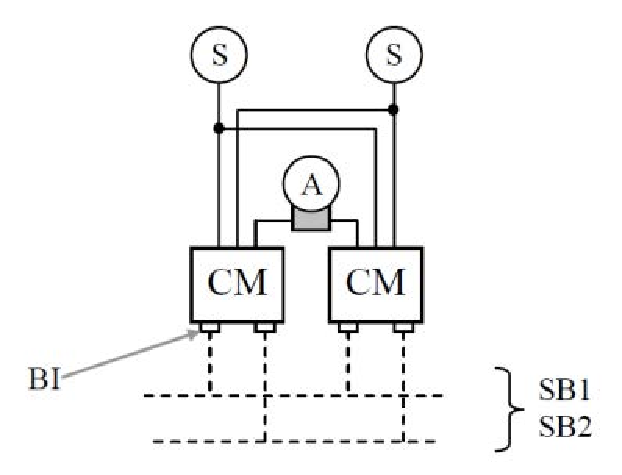
\includegraphics[scale=0.7]{Fig2.pdf}
  \caption{Wheel Unit}
  \label{fig2}
\end{figure}
\begin{figure}[H]
  \centering
  
\includegraphics[scale=1]{Fig3.pdf}
  \caption{Reliability block diagram of the wheel unit}
  \label{fig3}
\end{figure}
%--------------------------------
\subsection{Wheel Unit Subsystem Model}
/text/
\begin{figure}[H]
  \centering
  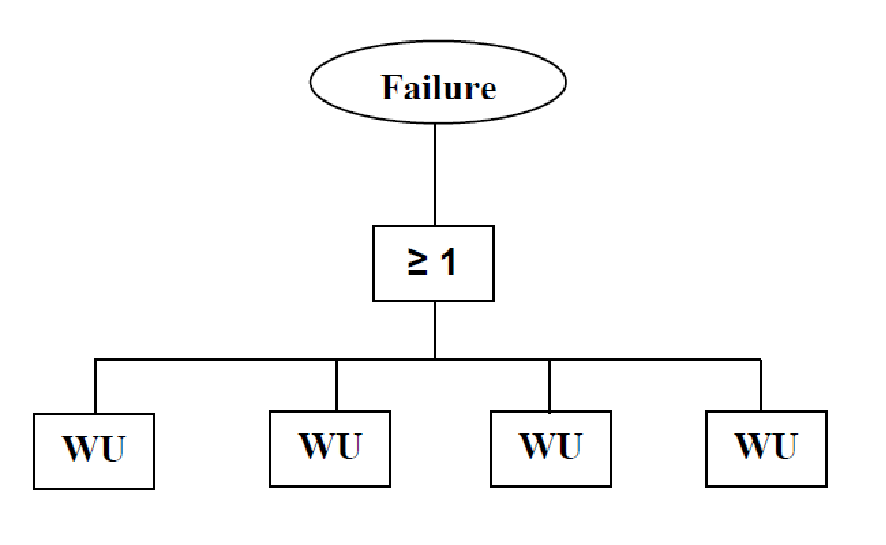
\includegraphics[scale=0.5]{Fig4.pdf}
  \caption{Fault tree for the Wheel Unit Subsystem, full functionality}
  \label{fig4}
\end{figure}
\begin{figure}[H]
  \centering
  
\includegraphics[scale=0.5]{Fig5.pdf}
  \caption{Fault tree for the Wheel Unit Subsystem, degraded functionality}
  \label{fig5}
\end{figure}
%--------------------------------
\subsection{Central Unit (CU)}
\subsubsection{Distributed Duplex Architecture}
\begin{figure}[H]
  \centering
  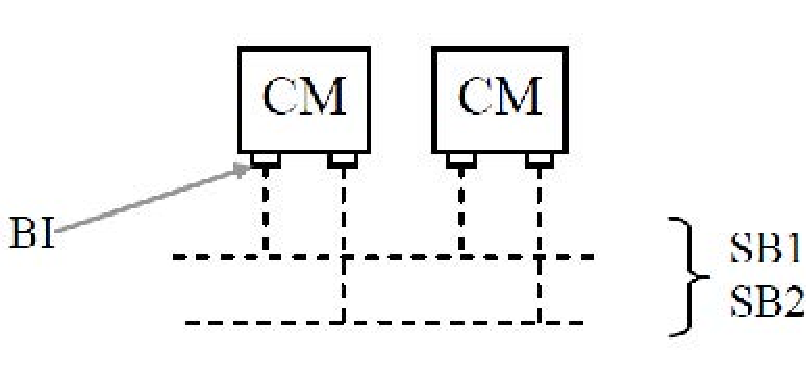
\includegraphics[scale=.5]{Fig6.pdf}
  \caption{Central Unit, duplex configuration }
  \label{fig6}
\end{figure}
\begin{figure}[H]
  \centering
  
\includegraphics[scale=.5]{Fig7.pdf}
  \caption{Reliability block diagram for the Central Unit, duplex configuration}
  \label{fig7}
\end{figure}
%The markov model for central unit-duplex is given below as an example. 
%\begin{figure}[h!]
%  \centering
%  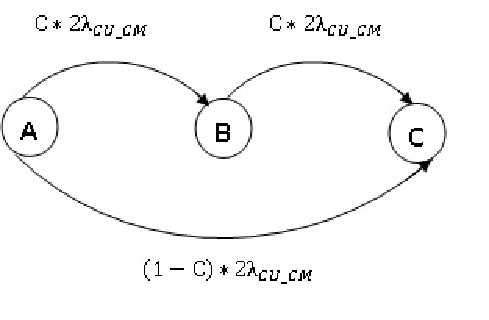
\includegraphics[scale=.7]{Fig8.pdf}
%  \caption{Markov model for the Central Unit. duplex configuration}
%  \label{fig8}
%\end{figure}
\begin{figure}[h!]
\begin{center}
\begin{tikzpicture}[node distance=5mm and 20mm]
\node[state] (s2) {A};
\node[state] (s3) [right= of s2] {B};
\node[state] (s4) [right= of s3] {C};
\draw [->,bend left=45] (s2) to node[above] {$c*2\lambda_{CU-CM} $} (s3);
\draw [->,bend right=45] (s2) to node[above] {$(1-c)*2\lambda_{CU-CM}$} (s4);
\draw [->,bend left=45] (s3) to node[above] {$\lambda_{CU-CM}$} (s4);
\end{tikzpicture}
\caption{Markov chain model}
\end{center}
\end{figure}
%-------------
\subsubsection{Centralized Triplex Architecture}

\begin{figure}[H]
  \centering
  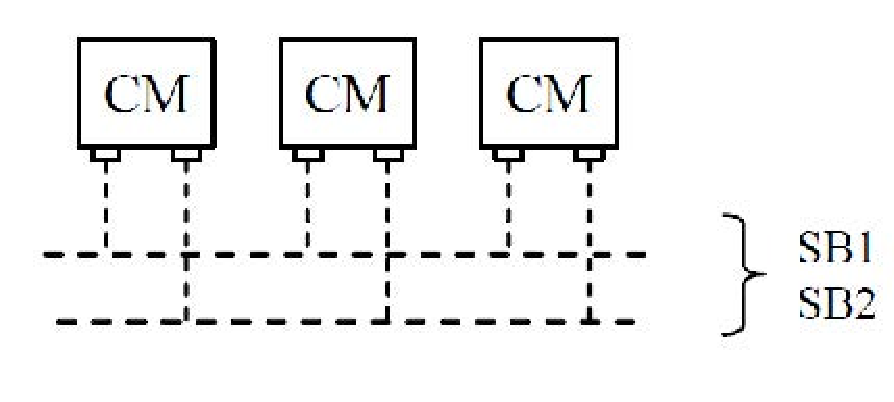
\includegraphics[scale=.5]{Fig9.pdf}
  \caption{Central Unit, triplex configuration }
  \label{fig9}
\end{figure}
/{Reliability block diagram for …, Figure 10.  Make sure the caption number is correct.}/
\\/{Markov model for …, Figure 11.}/

\begin{figure}[H]
  \centering
  
\includegraphics[scale=.5]{Fig10.pdf}
  \caption{Caption }
  \label{fig10}
\end{figure}
\begin{figure}[H]
  \centering
  
\includegraphics[scale=.5]{Fig11.pdf}
  \caption{Caption}
  \label{fig11}
\end{figure}
%--------------------------------
\subsection{System Model}
\subsubsection{Centralized Architecture}

\begin{figure}[H]
  \centering
  
\includegraphics[scale=.5]{Fig12.pdf}
  \caption{Fault tree for Full Functionality}
  \label{fig12}
\end{figure}
\begin{figure}[H]
  \centering
  
\includegraphics[scale=.5]{Fig13.pdf}
  \caption{Fault tree for Degraded Functionality}
  \label{fig13}
\end{figure}
%-------------
\subsubsection{Distributed Architecture}
\begin{figure}[H]
  \centering
  
\includegraphics[scale=.5]{Fig14.pdf}
  \caption{Fault tree for Full Functionality}
  \label{fig14}
\end{figure}
\begin{figure}[H]
  \centering
  
\includegraphics[scale=.5]{Fig15.pdf}
  \caption{Fault tree for Degraded Functionality}
  \label{fig15}
\end{figure}